\documentclass[11pt,a4paper]{article}
\usepackage[utf8]{inputenc}
\usepackage[french]{babel}
\usepackage[T1]{fontenc}

\usepackage{amsmath}
\usepackage{amsfonts}
\usepackage{amssymb}

\newcommand{\NomAuteur}{Fabrice BOISSIER}
\newcommand{\TitreMatiere}{Architecture des Ordinateurs}
\newcommand{\NomUniv}{EPITA - Bachelor Cyber Sécurité}
\newcommand{\NiveauUniv}{CYBER1}
\newcommand{\NumGroupe}{CYBER1}
\newcommand{\AnneeUniv}{2022-2023}
\newcommand{\DateExam}{janvier 2023}
\newcommand{\TypeExam}{Partiel (Sujet 1)}
\newcommand{\TitreExam}{\TitreMatiere}
\newcommand{\DureeExam}{2h00}
\newcommand{\MyWaterMark}{\AnneeUniv} % Watermark de protection

% Ajout de mes classes & definitions
\usepackage{MetalExam} % Appelle un .sty

% "Tableau" et pas "Table"
\addto\captionsfrench{\def\tablename{Tableau}}

%%%%%%%%%%%%%%%%%%%%%%%
%Header
%%%%%%%%%%%%%%%%%%%%%%%
\lhead{\TypeExam}							%Gauche Haut
\chead{\NomUniv}							%Centre Haut
\rhead{\NumGroupe}							%Droite Haut
\lfoot{\DateExam}							%Gauche Bas
\cfoot{\thepage{} / \pageref*{LastPage}}	%Centre Bas
\rfoot{\texttt{\TitreMatiere}}				%Droite Bas

%%%%%

\usepackage{tabularx}

\newlength{\LabelWidth}%
%\setlength{\LabelWidth}{1.3in}%
\setlength{\LabelWidth}{1cm}%
%\settowidth{\LabelWidth}{Employee E-mail:}%  Specify the widest text here.

% Optional first parameter here specifies the alignment of
% the text within the \makebox.  Default is [l] for left
% alignment. Other options are [r] and [c] for right and center
\newcommand*{\AdjustSize}[2][l]{\makebox[\LabelWidth][#1]{#2}}%


\definecolor{mGreen}{rgb}{0,0.6,0}
\definecolor{mGray}{rgb}{0.5,0.5,0.5}
\definecolor{mPurple}{rgb}{0.58,0,0.82}
\definecolor{backgroundColour}{rgb}{0.95,0.95,0.92}

\lstdefinestyle{CStyle}{
    backgroundcolor=\color{backgroundColour},
    commentstyle=\color{mGreen},
    keywordstyle=\color{magenta},
    numberstyle=\tiny\color{mGray},
    stringstyle=\color{mPurple},
    basicstyle=\footnotesize,
    breakatwhitespace=false,
    breaklines=true,
    captionpos=b,
    keepspaces=true,
    numbers=left,
    numbersep=5pt,
    showspaces=false,
    showstringspaces=false,
    showtabs=false,
    tabsize=2,
    language=C
}


\hyphenation{op-tical net-works SIGKILL}


\begin{document}

%\MakeExamTitleDuree     % Pour afficher la duree
\MakeExamTitle                   % Ne pas afficher la duree

%% \MakeStudentName    %% A reutiliser sur chaque nouvelle page

\bigskip
%\bigskip

Vous devez respecter les consignes suivantes, sous peine de 0 :

\begin{itemize}
\item Lisez le sujet en entier avec attention
\item Répondez sur le sujet
\item Ne détachez pas les agrafes du sujet
\item \'Ecrivez lisiblement vos réponses (si nécessaire en majuscules)
\item Les appareils électroniques sont tous interdits (calculatrices également)
\item Ne trichez pas
\end{itemize}

%\bigskip

\vfillFirst

% Questions cours
\section{Questions (8 points)}

\subsection{(1 point) Rappelez les 14 premières puissances de 2 : }

\bigskip


\begin{table}[ht!]
\centerline{
\begin{tabular}{ | m{0.5cm} | m{0.5cm} | m{0.5cm} | m{0.5cm} | m{0.65cm} | m{0.65cm} | m{0.65cm} | m{1cm} | m{1cm} | m{1cm} | m{1.5cm} | m{1.5cm} | m{1.5cm} | m{1.5cm} |}
\hline
$ 2^{0} $ & $ 2^{1} $ & $ 2^{2} $ & $ 2^{3} $ & $ 2^{4} $ & $ 2^{5} $ & $ 2^{6} $ & $ 2^{7} $ & $ 2^{8} $ & $ 2^{9} $ & $ 2^{10} $ & $ 2^{11} $ &  $ 2^{12} $ &  $ 2^{13} $ \\
\hline
 & & & & & & & & & & & & & \\
 & & & & & & & & & & & & & \\
 & & & & & & & & & & & & & \\
\hline
\end{tabular}
}
\end{table}


\bigskip

\subsection{(4 points) Convertissez ces nombres en décimaux. Vous donnerez leur interprétation non-signée puis signée.}

\bigskip

\centerline{
\begin{tabular}{ c |  m{2cm}   c   m{2cm} | m{2cm}   c   m{2cm} }
                                & & non-signé & & & signé & \\
 & & & &  & & \\
\hline
 & & & &  & & \\
$ \% \, 1101 \; 0101 \; 0110 $  & &           & & &  & \\
 & & & &  & & \\
\hline
% & & & &  & & \\
%$ \% \, 1110 \; 1001 \; 0011 $  & &           & & &  & \\
% & & & &  & & \\
%\hline
 & & & &  & & \\
$ \% \, 1010 \; 0001 \; 1100 $  & &           & & &  & \\
 & & & &  & & \\
\hline
% & & & &  & & \\
%\$ ACD  & &           & & &  & \\
% & & & &  & & \\
%\hline
 & & & &  & & \\
\$ 9BD  & &           & & &  & \\
 & & & &  & & \\
\hline
 & & & &  & & \\
\$ A66  & &           & & &  & \\
 & & & &  & & \\
\end{tabular}
}

% \bigskip

\vfillLast

\newpage

\subsection{(3 points) Convertissez ces nombres décimaux en binaire sur 12 bits, puis en hexadécimal.}

\bigskip

\centerline{
\begin{tabular}{ c |  m{2cm}   c   m{2cm} | m{2cm}   c   m{2cm} }
                                & & binaire & & & hexadécimal & \\
 & & & &  & & \\
\hline
 & & & &  & & \\
$ 42 $    & &           & & &  & \\
 & & & &  & & \\
\hline
% & & & &  & & \\
%$ 1664 $  & &           & & &  & \\
% & & & &  & & \\
%\hline
 & & & &  & & \\
$ 4321 $  & &           & & &  & \\
 & & & &  & & \\
\hline
 & & & &  & & \\
$ -116 $   & &          & & &  & \\
 & & & &  & & \\
\end{tabular}
}

\bigskip

\bigskip

\subsection{(2 points) Convertissez ces nombres en flottants au format IEEE 754 simple précision : }

\bigskip

\centerline{
\begin{tabular}{| c ||  c |C{0.33cm}|C{0.33cm}|C{0.33cm}|C{0.33cm}|C{0.33cm}|C{0.33cm}|C{0.33cm}|C{0.33cm}   ||  c |C{0.33cm}|C{0.33cm}|C{0.33cm}|C{0.33cm}|C{0.33cm}|C{0.33cm}|C{0.33cm}|C{0.33cm}|C{0.33cm}| }
\hline
                                          & \multicolumn{9}{c||}{\multirow{2}{*}{exposant}}   & \multicolumn{9}{c|}{\multirow{2}{*}{hexadécimal}} \\
                                          & \multicolumn{9}{c||}{ }                           & \multicolumn{9}{c|}{ } \\
\hline
\multirow[c]{3}{*}[0in]{$ 68,78125 $}     & \multirow[c]{3}{*}[0in]{$ \% $} & & & & & & & &  & \multirow[c]{3}{*}[0in]{$ \$ $} & & & & & & & & \\
                                          & & & & & & & & &                                  & & & & & & & & & \\
                                          & & & & & & & & &                                  & & & & & & & & & \\
\hline
\multirow[c]{3}{*}[0in]{$ -218,3203125 $} & \multirow[c]{3}{*}[0in]{$ \% $} & & & & & & & &  & \multirow[c]{3}{*}[0in]{$ \$ $} & & & & & & & & \\
                                          & & & & & & & & &                                  & & & & & & & & & \\
                                          & & & & & & & & &                                  & & & & & & & & & \\
\hline
\end{tabular}
}


\bigskip

\bigskip

\bigskip


\vfillFirst

\begin{center}
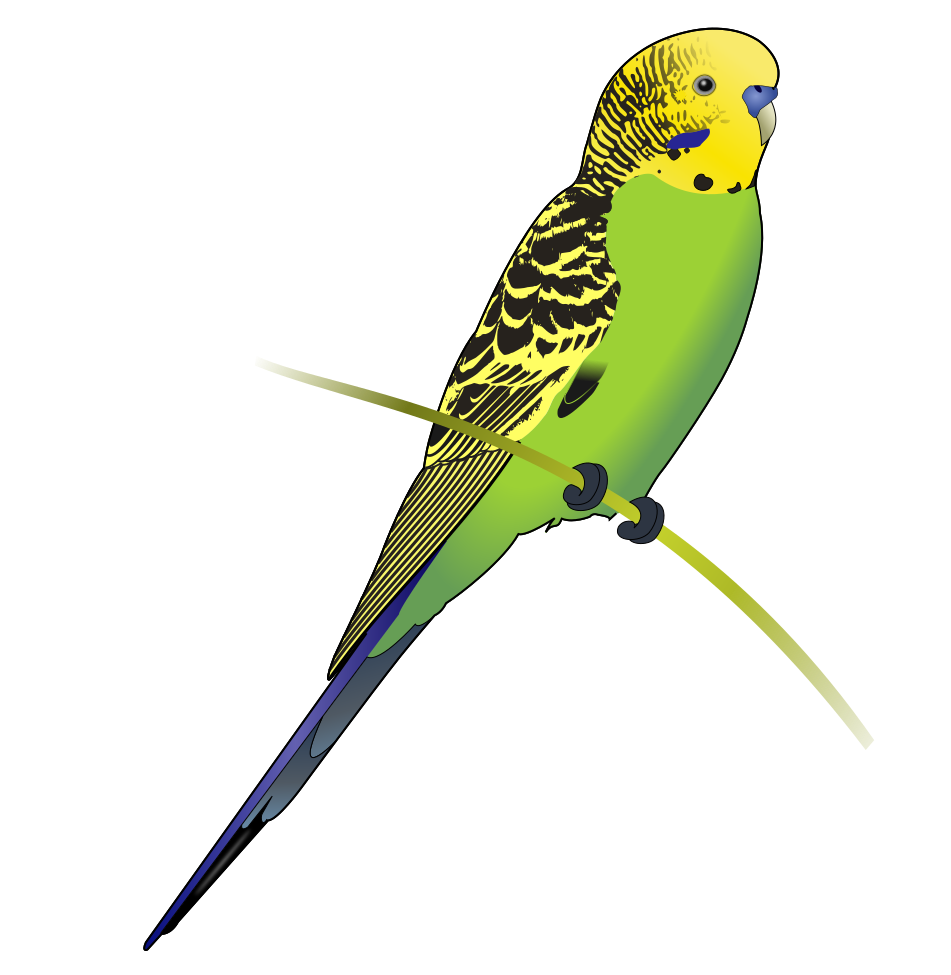
\includegraphics[scale=0.2]{img/others/Budgerigar_diagram.png}
\end{center}

\vfillLast

\clearpage

%%%%%%%%%%%%%%%%%%%%%%%%%%%%%%%%%%%%%%%%%%%%%%%%%%%%%%%
%%%%%%%%%%%%%%%%%%%%%%%%%%%%%%%%%%%%%%%%%%%%%%%%%%%%%%%
%%%%%%%%%%%%%%%%%%%%%%%%%%%%%%%%%%%%%%%%%%%%%%%%%%%%%%%

\section{Problème (10 points)}

%Un stagiaire de l'équipe système et sécurité (anciennement le LSE) a eu la mauvaise surprise de voir son ordinateur stoppé durant la séquence de boot (le démarrage du système d'exploitation).
%En redémarrant son ordinateur, un message s'affiche à l'écran : \og \texttt{No boot option} \fg{}.
%Visiblement, le disque dur n'est plus totalement reconnu, mais les données sont encore accessibles.
%Vous allez tenter de les récupérer manuellement.

Afin de vous plonger réellement dans le \textit{forensic} (analyse forensique ou investigation numérique en français), une toute petite FAT12 a été réalisée et utilisée pour produire quelques fichiers et dossiers contenant quelques mots.
L'objectif est de retrouver ce contenu.

\smallskip

Cet exercice a été réalisé avec une série de commandes que vous pourrez réaliser de votre côté pour également observer l'évolution d'une petite FAT12 (voir \TTBF{truncate(1)}, \TTBF{mkfs(1)} et \TTBF{mount(1)}).
%Cependant, la plus petite FAT possible avec les outils linux reste une FAT12 de 50 kilo-octets, c'est-à-dire, toujours trop pour tenir sur une ou deux feuilles A4 en examen.
%N'oubliez pas d'utiliser \textit{ghex} (ou d'autres éditeurs hexadécimaux) régulièrement pour observer les changements d'état de la FAT lorsque vous expérimenterez chez vous.
%(voir \TTBF{touch(1)}, \TTBF{truncate(1)}, \TTBF{mkfs(1)}, \TTBF{mkfs.vfat(1)}, \TTBF{mount(1)}, \TTBF{mkdir(1)}, \TTBF{umount(1)}, \TTBF{ghex(1)})


% touch Disk.img
% truncate Disk.img -s 1M
% truncate Disk.img -s 50K

% FAT12  (50K minimum)
% mkfs.vfat -F12 Disk.img
%% options :
%% mkfs.vfat -F12 -S512 -s1 Disk.img

% FAT16
% mkfs -t fat /dev/sdc1
% mkfs.fat -F 16 -I /dev/sdc1

% FAT32
% mkfs.fat -F 32 -I /dev/sdc

% NTFS
% mkfs -t ntfs /dev/sdc1
% mkfs.ntfs /dev/sdc1

\bigskip

\begin{Large}
\textbf{Description du système de fichiers FAT}
\end{Large}

\bigskip

\noindent Le format FAT (\textit{File Allocation Table}) est relativement simple, mais de nombreux champs dans les structures ainsi que des régions ne seront pas utiles dans notre cas.
Une partition formatée en FAT12 ou 16 se divise en quatre régions :
\begin{itemize}
\item le secteur de boot contenant le BPB (BIOS Parameter Block)
\item une table d'allocation de fichiers (FAT en anglais), et sa copie de sauvegarde
\item la région du dossier racine (cette région n'existe pas en FAT32)
\item la région du contenu des fichiers et dossiers
\end{itemize}

%\medskip

\begin{center}
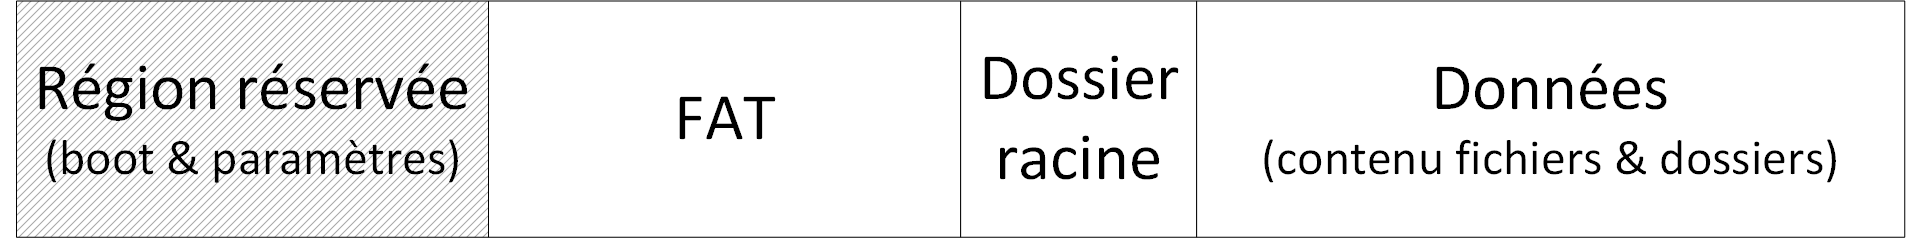
\includegraphics[width=12cm]{img/0-FAT_regions.png}
\end{center}

%\bigskip

\noindent La FAT (la deuxième région) est un tableau dont chaque numéro de case correspond à un cluster.

\begin{table}[ht!]
  \centering
  \begin{minipage}{0.50\textwidth}
    \centering

%\noindent La FAT (la deuxième région) est un tableau dont chaque numéro de case correspond à un cluster, et la valeur stockée dans la case indique si ce cluster est :
\noindent La valeur dans la case indique que le cluster est :
\begin{itemize}
\item libre (0x000)
\item abîmé/\textit{bad cluster} (0xFF7)
\item alloué (valeurs entre 0x002 et 0xFF5, ainsi que 0xFFF)
\end{itemize}

\medskip

%\begin{table}[ht!]
%  \centering
%  \begin{minipage}{0.50\textwidth}
%    \centering

%Ainsi, dans la FAT exemple suivante où chaque entrée prend 12 bits :
Pour chaque entrée de 12 bits dans la FAT :
\begin{itemize}
\item les clusters 3 et 7 sont libres,
\item les clusters 2 et 4 et 5 sont utilisés,
\item le cluster 6 est abîmé.
\end{itemize}

%\medskip

%Un fichier volumineux est stocké dans plusieurs clusters liés entre eux dans la FAT, comme une liste chaînée.
%Par exemple, en lisant les clusters 2, 5, puis 4 dans cet ordre précis, on obtiendrait le contenu d'un fichier.
%Le cluster 2 renvoie vers le 5, qui renvoie vers le 4, qui indique la fin (\texttt{0xFFF)}.
%%Pour reconstituer un fichier volumineux, les clusters sont chaînés entre eux, et la FAT catalogue les chaînes de clusters.
%%Ainsi, le contenu d'un fichier se trouve précisément dans ces clusters chaînés dans cet ordre : 2, 5, 4.

  \end{minipage}
  \hfillx
  \begin{minipage}{0.15\textwidth}

\begin{center}
\begin{tabular}{| l | l |}
\hline
\multicolumn{2}{| c |}{...} \\
\hline
FAT[2] & 0x005 \\
\hline
FAT[3] & 0x000 \\
\hline
FAT[4] & 0xFFF \\
\hline
FAT[5] & 0x004 \\
\hline
FAT[6] & 0xFF7 \\
\hline
FAT[7] & 0x000 \\
\hline
\multicolumn{2}{| c |}{...} \\
\hline
\end{tabular}
\end{center}

  \end{minipage}
  \hfillx
  \begin{minipage}{0.20\textwidth}

FAT exemple :
\begin{center}
\begin{lstlisting}[style=algorithmique]
   ...
00 50 00
FF F0 04
FF 70 00
   ...
\end{lstlisting}
\end{center}

  \end{minipage}
\end{table}

Un fichier volumineux est stocké dans plusieurs clusters liés entre eux dans la FAT, comme une liste chaînée.
Par exemple, en lisant les clusters 2, 5, puis 4 dans cet ordre précis, on obtiendrait le contenu d'un fichier.
Le cluster 2 renvoie vers le 5, qui renvoie vers le 4, qui indique la fin (\texttt{0xFFF)}.
%Pour reconstituer un fichier volumineux, les clusters sont chaînés entre eux, et la FAT catalogue les chaînes de clusters.
%Ainsi, le contenu d'un fichier se trouve précisément dans ces clusters chaînés dans cet ordre : 2, 5, 4.

%\bigskip
\medskip

Jusque là, nous avons vu comment retrouver le contenu des données stockées dans une partition formatée en FAT12.
%Concernant la différence entre un fichier et un dossier, et surtout, de retrouver leurs noms, il faut étudier les \textit{directory entries} (ou \textit{direntry}) : des structures de données contenant les caractéristiques des objets stockés dans la partition.
Pour identifier des fichiers et des dossiers parmi les données, il est nécessaire d'étudier les \textit{directory entries} (ou \textit{direntry}) : des structures de données contenant les caractéristiques des objets stockés dans la partition.

\medskip

Un dossier est littéralement un tableau contant des structures de données décrivant chacune un fichier ou un dossier.
Il y a donc autant de cases dans le tableau qu'il y a de fichiers et dossiers contenus à ce niveau hiérarchique.

\medskip

\begin{table}[ht!]
  \centering
  \begin{minipage}{0.3\textwidth}
%    \centering

\noindent \TTBF{dossier/} \\
\TTBF{dossier/fichier1} \\
\TTBF{dossier/fichier2} \\
\TTBF{dossier/fichier3} \\

  \end{minipage}
  \hfillx
  \begin{minipage}{0.6\textwidth}

\begin{lstlisting}[language=C,commentstyle=\color{commentgreen}]
struct direntry   entries[3]; // dossier
entries[0];       // dossier/fichier1
entries[1];       // dossier/fichier2
entries[2];       // dossier/fichier3 \end{lstlisting}

  \end{minipage}
%  \caption{Algorithme de la somme des N premiers entiers}
%  \label{somme-n-premiers-entiers}
\end{table}

\newpage

La structure représentant une \textit{direntry} est de la forme suivante.
On notera que FAT12 est très limité, ainsi, les fichiers ont des noms de 11 caractères maximum (8 avant l'extension, et 3 après).
%De plus, le champs \texttt{reserved\_and\_dates} cache en réalité de nombreux champs qui ne nous intéressent pas pour cet exercice.
\`A noter : la taille enregistrée dans le champs \textit{size} est en octets.

\begin{table}[ht!]
  \centering
  \begin{minipage}{0.51\textwidth}
    \centering
% %*   *)
% [style=algorithmique]

%\begin{lstlisting}[language=C]
%struct direntry {
%  char[11] name;
%  char     attributes;
%  char     reserved_1;
%  char     creation_time_s;
%  int      creation_time;
%  int      creation_date;
%  int      last_access_date;
%  char[2]  reserved_2;
%  int      last_modification_time;
%  int      last_modification_date;
%  int      first_cluster;
%  long     size;
%} __attribute__((packed)) \end{lstlisting}

\begin{lstlisting}[language=C]
struct direntry {
  char[11] name;
  char     attributes;
  char[14] reserved_and_dates;
  int      first_cluster;
  long     size;
} __attribute__((packed)) \end{lstlisting}

Taille en octets d'une \textit{direntry} : \_\_\_\_\_\_ \textit{(0,5 pts)}

  \end{minipage}
  \hfillx
  \begin{minipage}{0.39\textwidth}

Les types de données font :

\smallskip

\begin{tabular}{l l l l}
char & : & 1 octet  & (8 bits)  \\
int  & : & 2 octets & (16 bits) \\
long & : & 4 octets & (32 bits) \\
\end{tabular}

%\textit{Rappel : char[11] correspond à un tableau de 11 cases (de 0 à 10)}

\medskip

Attributs :

\medskip

\begin{tabular}{l l}
ATTR\_READ\_ONLY & 0x01 \\
ATTR\_HIDDEN     & 0x02 \\
ATTR\_SYSTEM     & 0x04 \\
ATTR\_VOLUME\_ID & 0x08 \\
ATTR\_DIRECTORY  & 0x10 \\
ATTR\_ARCHIVE    & 0x20 \\
\end{tabular}

  \end{minipage}
%  \caption{Algorithme de la somme des N premiers entiers}
%  \label{somme-n-premiers-entiers}
\end{table}

%\bigskip

\noindent Pour vous aider à retrouver les chaînes de caractères, une table ASCII décimale/caractères est fournie :

\begin{center}
\begin{tabular}{ | l |c|c|c|c|c| c |c|c|c|c|c|c|c|c|c|c| }
\hline
Dec &         10         &        13         &         32        & 45 & 46 &   & 48 & 49 & 50 & 51 & 52 & 53 & 54 & 55 & 56 & 57 \\
\hline
Char & \textbackslash{}n & \textbackslash{}r & \textit{(espace)} &  - &  . &   & 0 &  1 &  2 &  3 &  4 &  5 &  6 &  7 &  8 &  9 \\
\hline
\end{tabular}
%\end{center}

%\bigskip
\medskip

%\begin{center}
%\centerline{
%\begin{tabular}{ | l |c|c|c|c|c|c|c|c|c|c|c|c|c|c|c|c|c|c|c|c|c|c|c|c|c|c| }
%\hline
%Dec &  65 & 66 & 67 & 68 & 69 & 70 & 71 & 72 & 73 & 74 & 75 & 76 & 77 & 78 & 79 & 80 & 81 & 82 & 83 & 84 & 85 & 86 & 87 & 88 & 89 & 90 \\
%\hline
%Char &  A &  B &  C &  D &  E &  F &  G &  H &  I &  J &  K &  L &  M &  N &  O &  P &  Q &  R &  S &  T &  U &  V &  W &  X &  Y &  Z \\
%\hline
%\end{tabular}

\begin{tabular}{ | l |c|c|c|c|c|c|c|c|c|c|c|c|c| }
\hline
Dec &  65 & 66 & 67 & 68 & 69 & 70 & 71 & 72 & 73 & 74 & 75 & 76 & 77 \\
\hline
Char &  A &  B &  C &  D &  E &  F &  G &  H &  I &  J &  K &  L &  M \\
\hline
%\end{tabular}
%
%\smallskip
%
%\begin{tabular}{ | l |c|c|c|c|c|c|c|c|c|c|c|c|c| }
\hline
Dec &  78 & 79 & 80 & 81 & 82 & 83 & 84 & 85 & 86 & 87 & 88 & 89 & 90 \\
\hline
Char &  N &  O &  P &  Q &  R &  S &  T &  U &  V &  W &  X &  Y &  Z \\
\hline
\end{tabular}

%}

%\bigskip
\medskip

\begin{tabular}{ | l |c|c|c|c|c|c|c|c|c|c|c|c|c| }
\hline
Dec &  97 & 98 & 99 & 100 & 101 & 102 & 103 & 104 & 105 & 106 & 107 & 108 & 109 \\
\hline
Char &  a &  b &  c &  d  &  e  &  f  &  g  &  h  &  i  &  j  &  k  &  l  &  m \\
\hline
%\end{tabular}
%
%\smallskip
%
%\begin{tabular}{ | l |c|c|c|c|c|c|c|c|c|c|c|c|c| }
\hline
Dec &  110 & 111 & 112 & 113 & 114 & 115 & 116 & 117 & 118 & 119 & 120 & 121 & 122 \\
\hline
Char &  n  &  o  &  p  &  q  &  r  &  s  &  t  &  u  &  v  &  w  &  x  &  y  &  z \\
\hline
\end{tabular}

\end{center}

%\smallskip
%\medskip
%\newpage

%Le disque dur que l'on veut récupérer a apparemment été formaté en FAT12, c'est-à-dire que les fichiers ont un nom dont la taille est très limitée (8 caractères avant l'extension, et 3 après).

\subsection{(2 points) Première étape : séparation des champs du dossier racine }

Le dossier racine (ou \textit{root directory} en anglais) est le premier dossier dans lequel des fichiers et des dossiers peuvent se trouver.
La région du dossier racine contient en réalité une \textit{direntry} avec quelques valeurs spécifiques.

\medskip

En lisant la région du dossier racine, on extrait les données suivantes.
Recopiez les différents champs dans le tableau associé, sans les interpréter pour le moment.


\begin{table}[ht!]
  \centering
  \hspace*{-1.1cm}
  \begin{minipage}{0.37\textwidth}
    \centering
% %*   *)
\begin{lstlisting}[style=algorithmique]
53 45 43 52 45 54 20 20
54 58 54 20 00 AB 6E 60
2C 56 2C 56 00 00 6E 60
2C 56 03 01 1F 00 00 00
56 4F 49 54 55 52 45 53
20 20 20 10 00 00 76 60
2C 56 2C 56 00 00 76 60
2C 56 04 02 00 00 00 00
\end{lstlisting}
  \end{minipage}
  \hfillx
  \begin{minipage}{0.6\textwidth}
    \centering

%\begin{tabular}{ | c | C{4cm} | C{4cm} | }
%\hline
% & direntry 1 (f1) & direntry 2 (f2) \\
%\hline
% & & \\
%name & & \\
% & & \\
%\hline
% & & \\
%attributes & & \\
% & & \\
%\hline
% & & \\
%first\_cluster & & \\
% & & \\
%\hline
% & & \\
%size & & \\
% & & \\
%\hline
%\end{tabular}

\begin{tabular}{ | c |C{0.33cm}|C{0.33cm}|C{0.33cm}|C{0.33cm}|C{0.33cm}|C{0.33cm} | C{0.33cm}|C{0.33cm}|C{0.33cm}|C{0.33cm}|C{0.33cm}|C{0.33cm}| }
\hline
                         & \multicolumn{6}{c|}{direntry[0] (f1)} & \multicolumn{6}{c|}{direntry[1] (f2)} \\
\hline

\multirow[c]{4}{*}[0in]{name} &             & & & & &            &   & & & & & \\
                              &             & & & & &            &   & & & & & \\
\cline{2-13}
                              &             & & & & &            &   & & & & & \\
                              &             & & & & &            &   & & & & & \\
\hline

\multirow[c]{3}{*}[0in]{attributes} & \multicolumn{6}{c|}{ } & \multicolumn{6}{c|}{ } \\
                              & \multicolumn{6}{c|}{ } & \multicolumn{6}{c|}{ } \\
                              & \multicolumn{6}{c|}{ } & \multicolumn{6}{c|}{ } \\
\hline

\multirow[c]{3}{*}[0in]{first\_cluster} & \multicolumn{6}{c|}{ } & \multicolumn{6}{c|}{ } \\
                              & \multicolumn{6}{c|}{ } & \multicolumn{6}{c|}{ } \\
                              & \multicolumn{6}{c|}{ } & \multicolumn{6}{c|}{ } \\
\hline

\multirow[c]{3}{*}[0in]{size} & \multicolumn{6}{c|}{ } & \multicolumn{6}{c|}{ } \\
                              & \multicolumn{6}{c|}{ } & \multicolumn{6}{c|}{ } \\
                              & \multicolumn{6}{c|}{ } & \multicolumn{6}{c|}{ } \\
\hline
\end{tabular}

  \end{minipage}
%  \caption{Algorithme de la somme des N premiers entiers}
%  \label{somme-n-premiers-entiers}
\end{table}


%\bigskip
%\newpage

\subsection{(2 points) Deuxième étape : conversion des champs }

Maintenant que vous avez extrait les champs, il est nécessaire de les convertir pour obtenir des valeurs interprétables.
Convertissez de l'hexadécimal vers le décimal pour retrouver les caractères.

Concernant les noms de fichiers, les normes FAT12 et FAT16 précisent que les 8 premiers caractères servent à coder le nom du fichier, et les 3 derniers servent à coder l'extension.
Si un caractère correspond à un espace, laissez sa case vide.

\medskip

\begin{center}

%\begin{tabular}{ c   | m{0.45cm} | m{0.45cm} | m{0.45cm} | m{0.45cm} | m{0.45cm} | m{0.45cm} | m{0.45cm} | m{0.45cm} | c | m{0.45cm} | m{0.45cm} | m{0.45cm} | }
%\cline{2-9} \cline{11-13}
%                  & & & & & & & & &     & & & \\
%direntry 1 (f1)   & & & & & & & & &  .  & & & \\
%                  & & & & & & & & &     & & & \\
%\cline{2-9} \cline{11-13}
%                  & & & & & & & & &     & & & \\
%direntry 2 (f2)   & & & & & & & & &  .  & & & \\
%                  & & & & & & & & &     & & & \\
%\cline{2-9} \cline{11-13}
%\end{tabular}

\begin{tabular}{ c   | m{0.45cm} | m{0.45cm} | m{0.45cm} | m{0.45cm} | m{0.45cm} | m{0.45cm} | m{0.45cm} | m{0.45cm} | c | m{0.45cm} | m{0.45cm} | m{0.45cm} | }
\cline{2-9} \cline{11-13}
\multirow[c]{2}{*}[0in]{direntry[0] (f1)}  & & & & & & & & &     & & & \\
                                           & & & & & & & & &  .  & & & \\
\cline{2-9} \cline{11-13}
\multirow[c]{2}{*}[0in]{direntry[1] (f2)}  & & & & & & & & &     & & & \\
                                           & & & & & & & & &  .  & & & \\
\cline{2-9} \cline{11-13}
\end{tabular}

\end{center}

\smallskip

Retrouvez maintenant les attributs de chaque direntry, puis convertissez les entiers en valeurs décimales.

Avant de convertir les entiers, il faut savoir qu'en FAT, les entiers sont codés en \textit{little endian} (\textit{petit boutiste} en français), c'est-à-dire que les octets sont écrits au fur et à mesure du plus petit poids au plus grand.
Ainsi, si on écrivait \og 1337 \fg{} en little endian par paquets de un chiffre, on écrirait \og 7331 \fg{}, car 7 a le poids le plus petit (celui des unités), et 1 a le poids le plus fort (celui des milliers).
Pour effectuer les conversions d'entiers, vous devrez donc inverser l'ordre de lecture des \underline{octets} avant de les convertir (ainsi, \og BE 3F \fg{} doit être interprété comme \og 3F BE \fg{} avant d'être converti en décimal, \og AB CD EF \fg{} doit être interprété comme \og EF CD AB \fg{}, et ainsi de suite).

\smallskip

% $ \Box $
% $ \square $
\begin{center}
\centerline{
\begin{tabular}{ | c | C{5cm} | C{5cm} | L{2.3cm} L{1.8cm} | }
\hline
 & \multirow[c]{2}{*}[0in]{taille (en octets)} & \multirow[c]{2}{*}[0in]{numéro du premier cluster} & \multicolumn{2}{c|}{\multirow{2}{*}{attributs}} \\
 & & & & \\
\hline
\multirow[c]{3}{*}[0in]{direntry[0] (f1)} & &   & $ \Box $ Read Only    & $ \Box $ Hidden\\
                                          & &   & $ \Box $ Volume ID    & $ \Box $ System\\
                                          & &   & $ \Box $ Directory    & $ \Box $ Archive\\
\hline
\multirow[c]{3}{*}[0in]{direntry[1] (f2)} & &   & $ \Box $ Read Only    & $ \Box $ Hidden\\
                                          & &   & $ \Box $ Volume ID    & $ \Box $ System\\
                                          & &   & $ \Box $ Directory    & $ \Box $ Archive\\
\hline
\end{tabular}
}
\end{center}


%\newpage
\bigskip


\subsection{(1 point) Troisième étape : lecture d'un fichier }

L'une des direntry précédente a un nom particulièrement intéressant, et il est clair qu'une information importante se trouve dans le cluster pointé.
Voici les données extraites du cluster dont il est question.
Convertissez le message contenu dans le fichier, mais n'oubliez pas de vous arrêtez à la taille en octets indiquée par la direntry associée (c'est-à-dire f1).
Faites attention à la casse, c'est-à-dire aux majuscules et minuscules lorsque vous écrirez votre réponse.

\smallskip

\begin{table}[ht!]
  \centering
%  \hspace*{-1.1cm}
  \begin{minipage}{0.4\textwidth}
    \centering
% %*   *)
\begin{lstlisting}[style=algorithmique]
4C 65 20 73 65 63 72 65
74 20 61 20 63 68 65 72
63 68 65 72 20 65 73 74
20 45 50 49 54 41 0A 54
4F 50 20 65 63 6F 6C 65
00 00 00 00 00 00 00 00
00 00 00 00 00 00 00 00
\end{lstlisting}
  \end{minipage}
  \hfillx
  \begin{minipage}{0.45\textwidth}
    \centering

%\line(1,0){250}
%
%\medskip
%
%\line(1,0){250}
%
%\medskip
%
%\line(1,0){250}
%
%\medskip
%
%\line(1,0){250}
%
%\medskip

\begin{tabular}{ | m{0.45cm} | m{0.45cm} | m{0.45cm} | m{0.45cm}   |   m{0.45cm} | m{0.45cm} | m{0.45cm} | m{0.45cm} | }
\hline
 & & &   &   & & & \\
 & & &   &   & & & \\
\hline
 & & &   &   & & & \\
 & & &   &   & & & \\
\hline
 & & &   &   & & & \\
 & & &   &   & & & \\
\hline
 & & &   &   & & & \\
 & & &   &   & & & \\
\hline
 & & &   &   & & & \\
 & & &   &   & & & \\
\hline
\end{tabular}

  \end{minipage}
%  \caption{Algorithme de la somme des N premiers entiers}
%  \label{somme-n-premiers-entiers}
\end{table}




\subsection{(5 points) C'est reparti... }

Le message récupéré semble parfaitement clair, mais c'est trop simple pour être la réponse attendue.
La deuxième direntry dispose peut être de la réponse.
Le cluster pointé par celle-ci renvoie ces données, remplissez la structure qui devrait logiquement lui être adjointe.

\bigskip

\begin{table}[ht!]
  \centering
  \hspace*{-1.1cm}
  \begin{minipage}{0.37\textwidth}
    \centering
% %*   *)
\begin{lstlisting}[style=algorithmique]
2E 20 20 20 20 20 20 20
20 20 20 10 00 60 B0 4C
31 56 31 56 00 00 B0 4C
31 56 04 02 00 00 00 00
2E 2E 20 20 20 20 20 20
20 20 20 10 00 60 B0 4C
31 56 31 56 00 00 B0 4C
31 56 00 00 00 00 00 00
4D 31 20 20 20 20 20 20
54 58 54 20 00 06 BD 4C
31 56 31 56 00 00 BD 4C
31 56 05 02 0C 00 00 00
4D 32 20 20 20 20 20 20
54 58 54 20 00 BB C2 4C
31 56 31 56 00 00 C2 4C
31 56 06 02 0A 00 00 00
\end{lstlisting}
  \end{minipage}
  \hfillx
  \begin{minipage}{0.6\textwidth}
    \centering

\begin{tabular}{ | c |C{0.33cm}|C{0.33cm}|C{0.33cm}|C{0.33cm}|C{0.33cm}|C{0.33cm} | C{0.33cm}|C{0.33cm}|C{0.33cm}|C{0.33cm}|C{0.33cm}|C{0.33cm}| }
\hline
                        & \multicolumn{6}{c|}{direntry[0] (f11)} & \multicolumn{6}{c|}{direntry[1] (f12)} \\
\hline

\multirow[c]{2}{*}[0in]{name} &             & & & & &            &   & & & & & \\
%                              &             & & & & &            &   & & & & & \\
\cline{2-13}
%                              &             & & & & &            &   & & & & & \\
                              &             & & & & &            &   & & & & & \\
\hline

\multirow[c]{2}{*}[0in]{attributes} & \multicolumn{6}{c|}{ } & \multicolumn{6}{c|}{ } \\
                              & \multicolumn{6}{c|}{ } & \multicolumn{6}{c|}{ } \\
%                              & \multicolumn{6}{c|}{ } & \multicolumn{6}{c|}{ } \\
\hline

\multirow[c]{2}{*}[0in]{first\_cluster} & \multicolumn{6}{c|}{ } & \multicolumn{6}{c|}{ } \\
                              & \multicolumn{6}{c|}{ } & \multicolumn{6}{c|}{ } \\
%                              & \multicolumn{6}{c|}{ } & \multicolumn{6}{c|}{ } \\
\hline

\multirow[c]{2}{*}[0in]{size} & \multicolumn{6}{c|}{ } & \multicolumn{6}{c|}{ } \\
                              & \multicolumn{6}{c|}{ } & \multicolumn{6}{c|}{ } \\
%                              & \multicolumn{6}{c|}{ } & \multicolumn{6}{c|}{ } \\
\hline
\end{tabular}

\medskip

\begin{tabular}{ | c |C{0.33cm}|C{0.33cm}|C{0.33cm}|C{0.33cm}|C{0.33cm}|C{0.33cm} | C{0.33cm}|C{0.33cm}|C{0.33cm}|C{0.33cm}|C{0.33cm}|C{0.33cm}| }
\hline
                        & \multicolumn{6}{c|}{direntry[2] (f13)} & \multicolumn{6}{c|}{direntry[3] (f14)} \\
\hline

\multirow[c]{2}{*}[0in]{name} &             & & & & &            &   & & & & & \\
%                              &             & & & & &            &   & & & & & \\
\cline{2-13}
%                              &             & & & & &            &   & & & & & \\
                              &             & & & & &            &   & & & & & \\
\hline

\multirow[c]{2}{*}[0in]{attributes} & \multicolumn{6}{c|}{ } & \multicolumn{6}{c|}{ } \\
                              & \multicolumn{6}{c|}{ } & \multicolumn{6}{c|}{ } \\
%                              & \multicolumn{6}{c|}{ } & \multicolumn{6}{c|}{ } \\
\hline

\multirow[c]{2}{*}[0in]{first\_cluster} & \multicolumn{6}{c|}{ } & \multicolumn{6}{c|}{ } \\
                              & \multicolumn{6}{c|}{ } & \multicolumn{6}{c|}{ } \\
%                              & \multicolumn{6}{c|}{ } & \multicolumn{6}{c|}{ } \\
\hline

\multirow[c]{2}{*}[0in]{size} & \multicolumn{6}{c|}{ } & \multicolumn{6}{c|}{ } \\
                              & \multicolumn{6}{c|}{ } & \multicolumn{6}{c|}{ } \\
%                              & \multicolumn{6}{c|}{ } & \multicolumn{6}{c|}{ } \\
\hline
\end{tabular}

  \end{minipage}
%  \caption{Algorithme de la somme des N premiers entiers}
%  \label{somme-n-premiers-entiers}
\end{table}


\begin{center}

\begin{tabular}{ c   | m{0.45cm} | m{0.45cm} | m{0.45cm} | m{0.45cm} | m{0.45cm} | m{0.45cm} | m{0.45cm} | m{0.45cm} | c | m{0.45cm} | m{0.45cm} | m{0.45cm} | }
\cline{2-9} \cline{11-13}
\multirow[c]{2}{*}[0in]{direntry[0] (f11)}  & & & & & & & & &     & & & \\
                                            & & & & & & & & &  .  & & & \\
\cline{2-9} \cline{11-13}
\multirow[c]{2}{*}[0in]{direntry[1] (f12)}  & & & & & & & & &     & & & \\
                                            & & & & & & & & &  .  & & & \\
\cline{2-9} \cline{11-13}
\multirow[c]{2}{*}[0in]{direntry[2] (f13)}  & & & & & & & & &     & & & \\
                                            & & & & & & & & &  .  & & & \\
\cline{2-9} \cline{11-13}
\multirow[c]{2}{*}[0in]{direntry[3] (f14)}  & & & & & & & & &     & & & \\
                                            & & & & & & & & &  .  & & & \\
\cline{2-9} \cline{11-13}
\end{tabular}


\bigskip

\bigskip


\centerline{
\begin{tabular}{ | c | C{5cm} | C{5cm} | L{2.3cm} L{1.8cm} | }
\hline
 & \multirow[c]{2}{*}[0in]{taille (en octets)} & \multirow[c]{2}{*}[0in]{numéro du premier cluster} & \multicolumn{2}{c|}{\multirow{2}{*}{attributs}} \\
 & & & & \\
\hline
\multirow[c]{3}{*}[0in]{direntry[0] (f11)} & &   & $ \Box $ Read Only    & $ \Box $ Hidden\\
                                           & &   & $ \Box $ Volume ID    & $ \Box $ System\\
                                           & &   & $ \Box $ Directory    & $ \Box $ Archive\\
\hline
\multirow[c]{3}{*}[0in]{direntry[1] (f12)} & &   & $ \Box $ Read Only    & $ \Box $ Hidden\\
                                           & &   & $ \Box $ Volume ID    & $ \Box $ System\\
                                           & &   & $ \Box $ Directory    & $ \Box $ Archive\\
\hline
\multirow[c]{3}{*}[0in]{direntry[2] (f13)} & &   & $ \Box $ Read Only    & $ \Box $ Hidden\\
                                           & &   & $ \Box $ Volume ID    & $ \Box $ System\\
                                           & &   & $ \Box $ Directory    & $ \Box $ Archive\\
\hline
\multirow[c]{3}{*}[0in]{direntry[3] (f14)} & &   & $ \Box $ Read Only    & $ \Box $ Hidden\\
                                           & &   & $ \Box $ Volume ID    & $ \Box $ System\\
                                           & &   & $ \Box $ Directory    & $ \Box $ Archive\\
\hline
\end{tabular}
}

\end{center}


%\medskip
\newpage


\noindent Avec toutes les méta-données réunies jusqu'à maintenant concernant f1, f2, f11, f12, f13, f14, que déduisez-vous à propos de f11 et f12 ? (observez particulièrement les numéros de clusters)

\bigskip

\GrilleReponseN{8}

\bigskip

\noindent Finalement, il reste encore deux derniers clusters à convertir.
Attention à la taille des données, ainsi qu'aux majuscules et minuscules.

\begin{table}[ht!]
  \centering
%  \hspace*{-1.1cm}
  \begin{minipage}{0.4\textwidth}
    \centering
% %*   *)
\begin{lstlisting}[style=algorithmique]
56 65 67 61 2D 4D 69 73
73 79 6C 0A 6E 31 0A 00
\end{lstlisting}

\begin{lstlisting}[style=algorithmique]
43 68 6F 75 70 65 74 74
65 0A 00 00 00 00 00 00
\end{lstlisting}

  \end{minipage}
  \hfillx
  \begin{minipage}{0.45\textwidth}
    \centering

\begin{tabular}{ | m{0.45cm} | m{0.45cm} | m{0.45cm} | m{0.45cm}   |   m{0.45cm} | m{0.45cm} | m{0.45cm} | m{0.45cm} | }
\hline
 & & &   &   & & & \\
 & & &   &   & & & \\
\hline
 & & &   &   & & & \\
 & & &   &   & & & \\
\hline
\end{tabular}

\bigskip

\bigskip

\begin{tabular}{ | m{0.45cm} | m{0.45cm} | m{0.45cm} | m{0.45cm}   |   m{0.45cm} | m{0.45cm} | m{0.45cm} | m{0.45cm} | }
\hline
 & & &   &   & & & \\
 & & &   &   & & & \\
\hline
 & & &   &   & & & \\
 & & &   &   & & & \\
\hline
\end{tabular}

  \end{minipage}
%  \caption{Algorithme de la somme des N premiers entiers}
%  \label{somme-n-premiers-entiers}
\end{table}



\begin{center}
\rule{\linewidth}{1pt}
\end{center}



Les commandes ayant permis de produire et utiliser la FAT sont les suivantes :

\begin{lstlisting}[style=sh]
touch Disk.img
truncate Disk.img -s 50K
# FAT12, secteurs de 512o, 1 secteur par cluster
mkfs.vfat -F12 -S512 -s1 Disk.img
sudo mount Disk.img /mnt
### ... ###
cd /
sudo umount /mnt \end{lstlisting}


Cependant, la plus petite FAT possible avec les outils linux reste une FAT12 de 50 kilo-octets, c'est-à-dire, toujours trop pour tenir sur une ou deux feuilles A4 en examen.
N'oubliez pas d'utiliser \textit{ghex} (ou d'autres éditeurs hexadécimaux) régulièrement pour observer les changements d'état de la FAT lorsque vous expérimenterez chez vous.
%(voir \TTBF{touch(1)}, \TTBF{truncate(1)}, \TTBF{mkfs(1)}, \TTBF{mkfs.vfat(1)}, \TTBF{mount(1)}, \TTBF{mkdir(1)}, \TTBF{umount(1)}, \TTBF{ghex(1)})



%\vfillFirst
%
%\begin{center}
%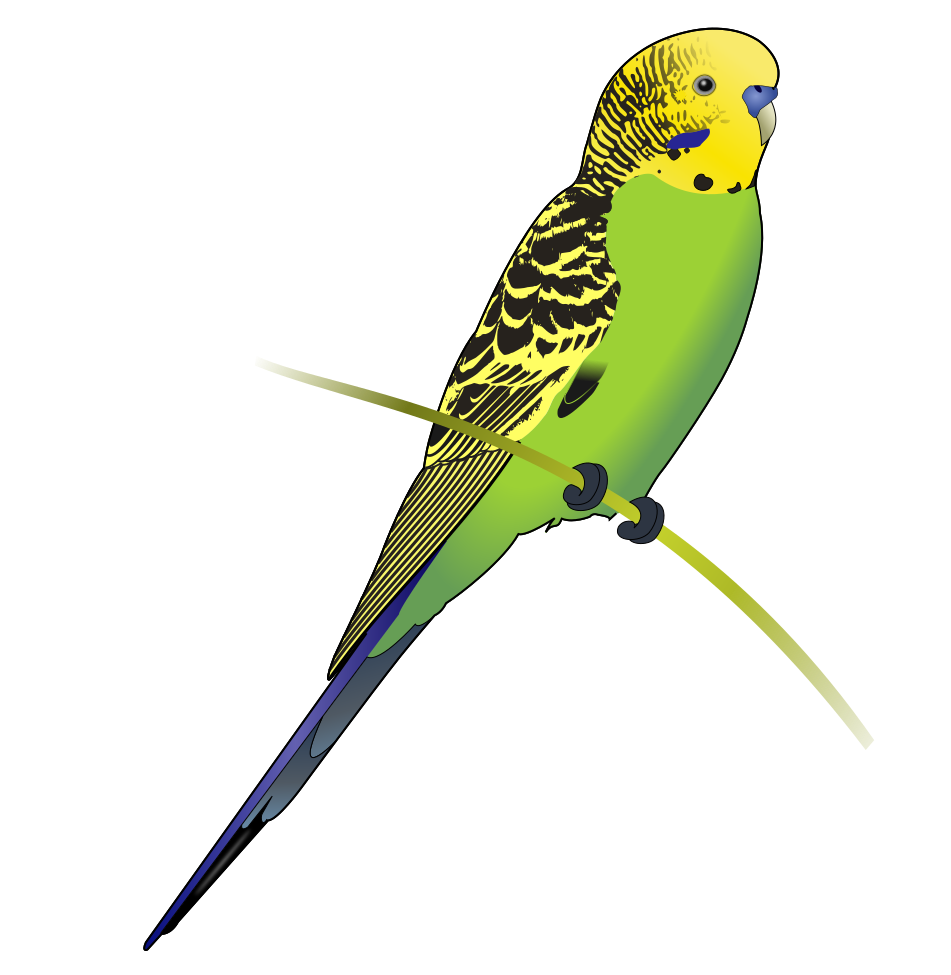
\includegraphics[scale=0.2]{img/others/Budgerigar_diagram.png}
%\end{center}
%
%\vfillLast


\newpage


%\thispagestyle{empty}

\vfillFirst

\begin{center}

\begin{LARGE}
\textbf{SUJET 1}
\end{LARGE}

\end{center}

\vfillLast

\end{document}
